% Hlavicka pro protokoly z fyzikalniho praktika.
% Verze pro: LaTeX
% Verze hlavicky: 22. 2. 2007
% Autor: Ustav fyziky kondenzovanych latek
% Ke stazeni: www.physics.muni.cz/ufkl/Vyuka/
% Licence: volne k pouziti, nejlepe k vcasnemu odevzdani protokolu z Vaseho mereni.


\documentclass[czech,11pt,a4paper]{article}
\usepackage[T1]{fontenc}
\usepackage{graphicx}
\usepackage{mathtools}
\usepackage{amssymb}
\usepackage{amsthm}
\usepackage{thmtools}
\usepackage{xcolor}
\usepackage{nameref}
\usepackage{babel}
\usepackage{hyperref}
\usepackage{multicol}
\usepackage[export]{adjustbox}
\usepackage{subcaption}
\usepackage{caption}
\usepackage{multirow}
\usepackage{float}
\usepackage{placeins}




%%% Nemente:
\usepackage[margin=2cm]{geometry}
\newtoks\jmenopraktika \newtoks\jmeno \newtoks\datum
\newtoks\obor \newtoks\skupina \newtoks\rocnik \newtoks\semestr
\newtoks\cisloulohy \newtoks\jmenoulohy
\newtoks\tlak \newtoks\teplota \newtoks\vlhkost
%%% Nemente - konec.


%%%%%%%%%%% Doplnte pozadovane polozky:

\jmenopraktika={Fyzikální praktikum 1}  % nahradte jmenem vaseho predmetu
\jmeno={Teodor Duraković}            % nahradte jmenem mericiho
\datum={6.~března 2024}        % nahradte datem mereni ulohy
\obor={F}                     % nahradte zkratkou vami studovaneho oboru
\skupina={St 8:00}            % nahradte dobou vyuky vasi seminarni skupiny
\rocnik={I}                  % nahradte rocnikem, ve kterem studujete
\semestr={II}                 % nahradte semestrem, ve kterem studujete

\cisloulohy={2}               % nahradte cislem merene ulohy
\jmenoulohy={Měření odporu rezistoru} % nahradte jmenem merene ulohy

\tlak={99 \,\rm 000}                   % nahradte tlakem pri mereni (v hPa)
\teplota={20.4}               % nahradte teplotou pri mereni (ve stupnich Celsia)
\vlhkost={42.3}               % nahradte vlhkosti vzduchu pri mereni (v %)

%%%%%%%%%%% Konec pozadovanych polozek.


%%%%%%%%%%% Uzitecne balicky:

%%%%%% Zamezeni parchantu:
\widowpenalty 10000 \clubpenalty 10000 \displaywidowpenalty 10000
%%%%%% Parametry pro moznost vsazeni vetsiho poctu obrazku na stranku
\setcounter{topnumber}{3}	  % max. pocet floatu nahore (specifikace t)
\setcounter{bottomnumber}{3}	  % max. pocet floatu dole (specifikace b)
\setcounter{totalnumber}{6}	  % max. pocet floatu na strance celkem
\renewcommand\topfraction{0.9}	  % max podil stranky pro floaty nahore
\renewcommand\bottomfraction{0.9} % max podil stranky pro floaty dole
\renewcommand\textfraction{0.1}	  % min podil stranky, ktery musi obsahovat text
\intextsep=8mm \textfloatsep=8mm  %\intextsep pro ulozeni [h] floatu a \textfloatsep pro [b] or [t]

% Tecky za cisly sekci:
\renewcommand{\thesection}{\arabic{section}.}
\renewcommand{\thesubsection}{\thesection\arabic{subsection}.}
% Jednopismenna mezera mezi cislem a nazvem kapitoly:
\makeatletter \def\@seccntformat#1{\csname the#1\endcsname\hspace{1ex}} \makeatother


%%%%%%%%%%%%%%%%%%%%%%%%%%%%%%%%%%%%%%%%%%%%%%%%%%%%%%%%%%%%%%%%%%%%%%%%%%%%%%%
%%%%%%%%%%%%%%%%%%%%%%%%%%%%%%%%%%%%%%%%%%%%%%%%%%%%%%%%%%%%%%%%%%%%%%%%%%%%%%%
% Zacatek dokumentu
%%%%%%%%%%%%%%%%%%%%%%%%%%%%%%%%%%%%%%%%%%%%%%%%%%%%%%%%%%%%%%%%%%%%%%%%%%%%%%%
%%%%%%%%%%%%%%%%%%%%%%%%%%%%%%%%%%%%%%%%%%%%%%%%%%%%%%%%%%%%%%%%%%%%%%%%%%%%%%%

\begin{document}
	
	%%%%%%%%%%%%%%%%%%%%%%%%%%%%%%%%%%%%%%%%%%%%%%%%%%%%%%%%%%%%%%%%%%%%%%%%%%%%%%%
	% Nemente:
	%%%%%%%%%%%%%%%%%%%%%%%%%%%%%%%%%%%%%%%%%%%%%%%%%%%%%%%%%%%%%%%%%%%%%%%%%%%%%%%
	\thispagestyle{empty}
	
	{
		\begin{center}
			\sf 
			{\Large Ústav fyzikální elektroniky Přírodovědecké fakulty Masarykovy univerzity} \\
			\bigskip
			{\huge \bfseries FYZIKÁLNÍ PRAKTIKUM} \\
			\bigskip
			{\Large \the\jmenopraktika}
		\end{center}
		
		\bigskip
		
		\sf
		\noindent
		\setlength{\arrayrulewidth}{1pt}
		\begin{tabular*}{\textwidth}{@{\extracolsep{\fill}} l l}
			\large {\bfseries Zpracoval:}  \the\jmeno & \large  {\bfseries Naměřeno:} \the\datum\\[2mm]
			\large  {\bfseries Obor:} \the\obor  \hspace{40mm}  {\bfseries Skupina:} \the\skupina %
			%{\bfseries Ročník:} \the\rocnik \hspace{5mm} {\bfseries Semestr:} \the\semestr  
			&\large {\bfseries Testováno:}\\
			\\
			\hline
		\end{tabular*}
	}
	
	\bigskip
	
	{
		\sf
		\noindent \begin{tabular}{p{3cm} p{0.6\textwidth}}
			\Large  Úloha č. {\bfseries \the\cisloulohy:} \par
			\smallskip
			$T=\the\teplota$~$^\circ$C \par
			$p=\the\tlak$~Pa \par
			$\varphi=\the\vlhkost$~\%
			&\Large \bfseries \the\jmenoulohy  \\[2mm]
		\end{tabular}
	}
	
	\vskip1cm
	
	%%%%%%%%%%%%%%%%%%%%%%%%%%%%%%%%%%%%%%%%%%%%%%%%%%%%%%%%%%%%%%%%%%%%%%%%%%%%%%%
	% konec Nemente.
	%%%%%%%%%%%%%%%%%%%%%%%%%%%%%%%%%%%%%%%%%%%%%%%%%%%%%%%%%%%%%%%%%%%%%%%%%%%%%%%
	
	%%%%%%%%%%%%%%%%%%%%%%%%%%%%%%%%%%%%%%%%%%%%%%%%%%%%%%%%%%%%%%%%%%%%%%%%%%%%%%%
	%%%%%%%%%%%%%%%%%%%%%%%%%%%%%%%%%%%%%%%%%%%%%%%%%%%%%%%%%%%%%%%%%%%%%%%%%%%%%%%
	% Zacatek textu vlastniho protokolu
	%%%%%%%%%%%%%%%%%%%%%%%%%%%%%%%%%%%%%%%%%%%%%%%%%%%%%%%%%%%%%%%%%%%%%%%%%%%%%%%
	%%%%%%%%%%%%%%%%%%%%%%%%%%%%%%%%%%%%%%%%%%%%%%%%%%%%%%%%%%%%%%%%%%%%%%%%%%%%%%%
	
	
	\section{Zadání}
	Zjistit odpor dvou rezistorů a voltampérovou charakteristiku žárovky dvěma různými metodami zapojení měřících přístrojů.
	
	\section{Postup, metody měření}
	Napětí měříme přístrojem Keysight U3402A, proud přístrojem Metex M-3850. Kromě samotného změřeného odporu, toto praktikum slouží i k experimentálnímu potvrzení pravidel, kdy jednotlivé metody použít.
	
	\begin{figure} [h]
		\begin{subfigure}{1\textwidth}
			\begin{center}
				
			\begin{tabular}{||c|c|c|c|c||}
				\hline
				& Rozsah & rozlišení & přesnost [\% rdg + dg] & vnitřní odpor\\
				\hline
				\multirow {3}{*}{Voltmetr} &$1.20000 \,\rm V $& $1 . 10^{-5} \,\rm V$  & $\pm \, 0.012\, \%   +5$ & $10.0 \,\rm M \Omega$ \\
				
				& $12.0000 \,\rm V $& $1 . 10^{-4} \,\rm V$  & $\pm \, 0.012 \, \%   +5$ & $11.1 \,\rm M \Omega$\\
				
				
				& $120.000 \,\rm V $& $1 . 10^{-3} \,\rm V$  & $\pm \, 0.012 \, \%   +5$ & $10.1 \,\rm M \Omega$\\
				\hline
				\multirow {2}{*}{Ampérmetr} &$0.040 \,\rm A $& $1 . 10^{-5} \,\rm A$  & $\pm \, 0.8\, \%   +1$ & $5.3 \,\rm  \Omega$ \\
				&$0.400 \,\rm A $& $1 . 10^{-4} \,\rm A$  & $\pm \, 0.8\, \%   +1$ & $5.3 \,\rm  \Omega$ \\
				
				& $20 \,\rm  A$& $1 . 10^{-2} \,\rm A$  & $\pm \, 1.5 \, \%   +5 $ & $5.3 \,\rm  \Omega$\\
				\hline
				
			\end{tabular}
			\end{center}
			
			\caption*{Parametry používaných rozsahů měřících přístrojů}
		\end{subfigure}
	\end{figure}
	\newpage
	
	\subsection{Metody měření}
	Měřící přístroje můžeme zapojit dvěma způsoby. Voltmetr sériově a ampérmetr paralelně, nebo naopak:

   
   \begin{figure}[H]
   	
   	\begin{subfigure}{0.5\textwidth}
   		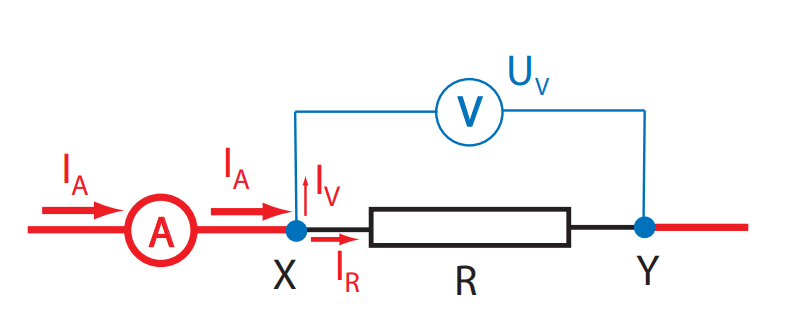
\includegraphics[width=0.9\linewidth, ]{MetodaA} 
   		\caption{Metoda A}
   		\label{fig:subim1}
   	\end{subfigure}
   	\begin{subfigure}{0.5\textwidth}
   		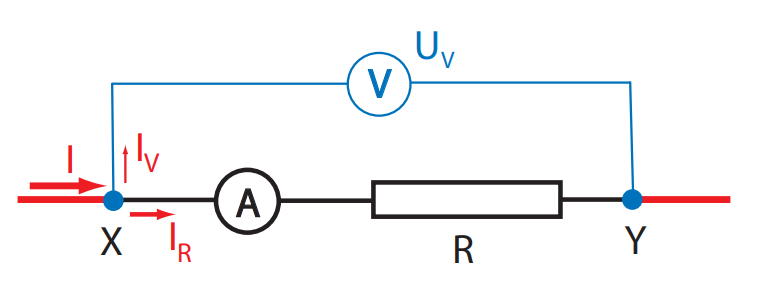
\includegraphics[width=0.9\linewidth, ]{MetodaB}
   		\caption{Metoda B}
   		\label{fig:subim2}
   	\end{subfigure}
   	
   	\caption{Schémata zapojení dle metod A a B}
   	\label{fig:image2} \end{figure}
   	
   	
   	
   	
   Oba způsoby zapojení do měření přinášejí systematickou chybu. Při metodě A měří ampérmetr proud, který se následně větví - neměří tedy pouze proud protékající rezistorem. Při metodě B ampérmetr měří sice správně, chyba je však tentokrát způsobena voltmetrem - ten měří kromě napětí na rezistoru i napětí na ampérmetru. \\
   Užitím vztahu \begin{equation}
   	R = \frac{U_V}{I_A}
   \end{equation}
   tedy dostaneme výsledek zatížený systematickou chybou.
   
   \subsubsection{Eliminace systematické chyby}
   Známe-li vnitřní odpory ampérmetru a voltmetru, můžeme při kalkulaci zmíněnou systematickou chybu odstranit, a to následujícím způsobem:
    \begin{figure}[h]
   	
   	\begin{subfigure}{0.5\textwidth}
   		\begin{center}
   			\begin{equation}
   					R = \frac{U_R}{I_R}=\frac{U_V}{I_A-I_V}= \frac{U_V}{I_A - \frac{U_V}{R_V}}
   			\end{equation}
   		\end{center}
   		\caption{Metoda A}
   	\end{subfigure}
   	\begin{subfigure}{0.5\textwidth}
   	\begin{center}
   	\begin{equation}
   			R = \frac{U_V - R_AI_A}{I_A} = \frac{U_V}{I_A}- R_A 
   		\end{equation}
   	\end{center}
   		\caption{Metoda B}
   	\end{subfigure}
   	 \end{figure}
   	 
   	 \subsection{Způsob kalkulace odporu}
	Měření odporu rezistorů jsou provedena každým způsobem jednou. Z těchto údajů je odpor vždy spočítán vztahem (1) i (2), resp. (3), v závislosti na způsobu zapojení měřících přístrojů.
	
	
	\section{Měření odporu rezistoru a kalkulace nejistot}
	Při měření odporu rezistoru byl voltmetr nastaven na rozsah $120\,\rm V$, ampérmetr byl nastaven na rozsah $400$, resp. $40 \,\rm mA$. Nejistotu spočítáme z odpovídajících řádků přesnosti. Získáváme tyto hodnoty: \\
	
	\begin{center}
		\begin{tabular}{||c|c|c|c|c||}
		\hline
		&   \multicolumn{2}{|c|}{Metoda A} & \multicolumn{2}{|c||}{Metoda B}  \\
		\hline
		& I [A] & U[V] & I[A] & U[V] \\
		\hline
		$R_1$ & $0.1913 \, \pm 0.0016 $ & $18.950\, \pm 0.007$ & $0.1927 \,\pm 0.0016$ & $ 20.125 \,\pm 0.007$ \\
		\hline
		$R_2$ &$ 3.10^{-5} \,\pm 1.10^{-5} $& $19.780 \,\pm 0.007$ & $3.10^{-5} \,\pm 1.10^{-5}$ & $20.135 \,\pm 0.007$ \\
		\hline
	\end{tabular}
	\end{center}
	
	\subsection{Nejistoty, výsledky}
	Zmíněné metody výpočtu provedeme v Pythonu s pomocí modulu \textit{uncertainties}, použijeme následující kód:
{\tiny 	\begin{verbatim}
		
		from uncertainties import ufloat
		R_V = ufloat(10.1*10**6, 0)
		R_A = ufloat(5.3, 0)
		U_1_A = ufloat(18.950, 0.007)
		I_1_A = ufloat(0.1913, 0.0016)
		#Metoda A, rezistor 1
		U_2_A = ufloat(19.780, 0.007)
		I_2_A = ufloat(3*10**(-5), 1*10**(-5))
		#Metoda A, rezistor 2
		
		U_1_B = ufloat(20.125, 0.007)
		I_1_B = ufloat(0.1927, 0.0016)
		#Metoda B, rezistor 1
		U_2_B = ufloat(20.135, 0.007)
		I_2_B = ufloat(3*10**(-5), 1*10**(-5))
		#Metoda B, rezistor 2
		
		R_1_A = U_1_A / I_1_A
		print("R1A = ",'{:.5u}'.format(R_1_A))
		R_1_A_kor = U_1_A / (I_1_A - (U_1_A / R_V))
		print("R1A - korekce= ", '{:.5u}'.format(R_1_A_kor))
		
		R_2_A = U_2_A / I_2_A
		print("R2A = ",'{:.5u}'.format(R_2_A))
		R_2_A_kor = U_2_A / (I_2_A - (U_2_A / R_V))
		print("R2A - korekce = ",'{:.5u}'.format(R_2_A_kor))
		
		R_1_B = U_1_B / I_1_B
		print("R1B = ",'{:.5u}'.format(R_1_B))
		R_1_B_kor = (U_1_B / I_1_B) - R_A
		print("R1B - korekce = ",'{:.5u}'.format(R_1_B_kor))
		
		R_2_B = U_2_B / I_2_B
		print("R2B = ",'{:.5u}'.format(R_2_B))
		R_2_B_kor = (U_2_B / I_2_B) - R_A
		print("R2B - korekce = ",'{:.5u}'.format(R_2_B_kor))
	\end{verbatim} }
	
	Získáváme tyto údaje:
	
	
	
	\begin{center}
		\begin{tabular}{||c|c|c|c|c||}
			\hline
			&   \multicolumn{2}{|c|}{Metoda A} & \multicolumn{2}{|c||}{Metoda B}  \\
			\hline
			& Bez korekce & S korekcí & Bez korekce & S korekcí \\
			\hline
			$R_1 [\Omega]$ & $99.059 \, \pm 0.83 $ & $99.060 \, \pm 0.83$ & $104.437 \,\pm 0.87$ & $ 99.137 \,\pm 0.87$ \\
			\hline
			$R_2 [\Omega]$ &$ 6,593.10^{5} \,\pm 2,198.10^{5} $& $ 7,054.10^5 \,\pm 2,516.10^5$ & $6,712.10^{5} \,\pm 2,237.10^{5}$ & $6,712.10^5 \,\pm 2,237.10^5$ \\
			\hline
		\end{tabular}
	\end{center}
	Hodnoty zde schválně nepodléhají správnému zaokrouhlení výsledku, jelikož by při něm rozdíly v~nejistotách jednotlivých metod nebyly viditelné. Z tabulky můžeme vidět, že nejmenší nejistota při správném počítání odporu (tj. s korekcí) je pro malý odpor u metody A a pro velký odpor u metody B.
	
	
	

	
	\section{Voltampérová charakteristika žárovky}
	Za předpokladu malého odporu žárovky jsme měřili pouze metodou A. Byla použita žárovka s maximálním napětím $12 \,\rm V$, proto jsme neměřili dle návodu v rozsahu $0-24\,\rm V$ Po prvním měření jsme se navíc spočítáním odporu přesvědčili, že má skutečně malou hodnotu. Získali jsme následující údaje:
	\begin{figure}[H]
			\begin{center}
				\begin{tabular}{l|l}
					U{[}V{]} & I{[}A{]} \\ \hline
					0.4946   & 0.01656  \\ \hline
					0.9095   & 0.02206  \\ \hline
					1.4250    & 0.02722  \\ \hline
					2.0715   & 0.03350   \\ \hline
					2.5850   & 0.03800    \\ \hline
					3.0215   & 0.0417  \\ \hline
					3.5695   & 0.0458   \\ \hline
					3.9656   & 0.0486   \\ \hline
					4.5535   & 0.0528   \\ \hline
					5.0393   & 0.0560   \\ \hline
					5.5102   & 0.0590    \\ \hline
					5.9950    & 0.0621   \\ \hline
					6.4340    & 0.0645   \\ \hline
					7.0160    & 0.0679   \\ \hline
					7.4430   & 0.0704   \\ \hline
					8.0039   & 0.0735   \\ \hline
					8.5157   & 0.0765   \\ \hline
					9.1447   & 0.0798   \\ \hline
					9.5600     & 0.0818   \\ \hline
					9.9250    & 0.0834   \\ \hline
					10.5165  & 0.0867   \\ \hline
					11.1100    & 0.0895   \\ \hline
					11.6760   & 0.0921  
				\end{tabular}
			\end{center}
		
	
	\end{figure}
	
	Ze kterých jsme vytvořili následující grafy:
	
	\begin{figure}[H]
		\begin{center}
			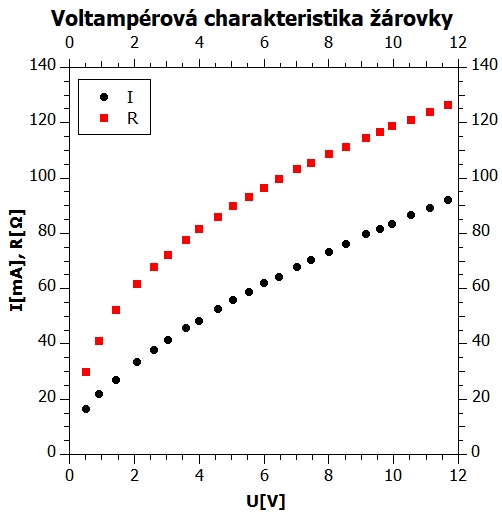
\includegraphics[width=0.5\textwidth]{VA_zarovka}
		\caption{Graf s vykreslenými hodnotami, závislost proudu a odporu na napětí}
		\includegraphics[width=0.5\textwidth]{Va_zarovka2}
		
		\caption{Graf s fitovanými polynomy 3. řádu pro R a I}
		\end{center}
	\end{figure}
	
	Po vykreslení hodnot je na první pohled vidět, že u žárovky závislost proudu na napětí \textbf{není} lineární. Fitovat graf přímkou by tudíž smysl nemělo, polynom 3. řádu se od hodnot již odchyluje minimálně. Nelinearita je zapříčiněna růstem odporu žárovky s rostoucí teplotou wolframového vlákna.
	

	
	
	
	
	\section{Závěr}
V dnešním praktiku jsme se dozvěděli, jak správně zapojit měřící přístroje v závislosti na odporu. \textit{}Dále jsme si potvrdili, nemůžeme vždy předpokládat konstantní odpor -to zejména v případě, kdy se vodič značně ohřívá.
	
	% Nakonec nezapomeňte projet text programem vlna nebo vlnka, např.
	% 	vlna -m -l -n mojeuloha.tex
	% nebo zkontrolovat a opravit jednopísmenné předložky na koncích řádků ručně.
	
	
\end{document}
